%!TEX root = paper.tex
\section{Results}

\indent{\indent Results of classification are evaluated on a micro-averaged F-score. Given the positive and negative rates for each class, the resulting score is computed the following way:}

\begin{equation}
    Precision_{micro} = \frac{\sum_{k \in C} TP_k}{\sum_{k \in C} TP_k + FP_k}, \;\;
    Recall_{micro} = \frac{\sum_{k \in C} TP_k}{\sum_{k \in C} TP_k + FN_k}
    \label{eq:PR}
\end{equation}

\begin{equation}
    F_{micro} = \frac{2*Precision_{micro}*Recall_{micro}}{Precision_{micro} + Recall_{micro}},
    \label{eq:mic_f1}
\end{equation}
where $C$ –– set of the plants classes

\vspace{1cm}

\indent{ The choice of such a metric is supported by the fact that classes are imbalanced. In this case, the influence of classes decreases due to averaging by classification characteristics, not by F-scores.}

\indent{The classificator output is shown on \ref{fig:metrics}}

\begin{figure}[h!]
	\centering
	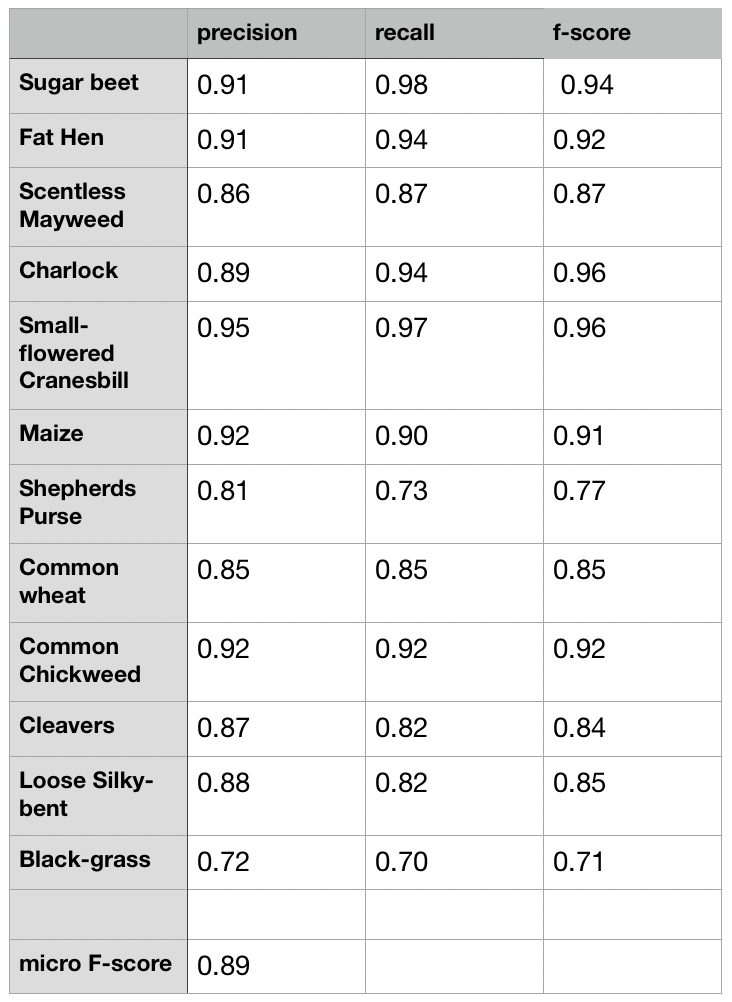
\includegraphics[width=7.cm, height=9.5cm]{metrics_1}
	\caption{Metric by class ant total metric}
	\label{fig:metrics}
\end{figure}